\begin{figure}[!h]


 \centering
 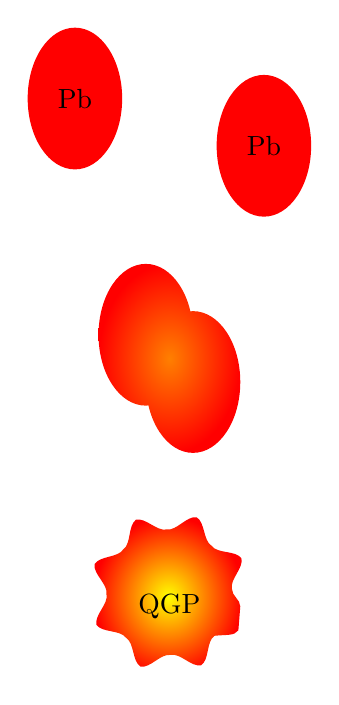
\begin{tikzpicture}[thick,scale=.3]

\fill[red] (0,23) ellipse (2 and 3) node [black,scale=1] {Pb};

\fill[red] (8,21) ellipse (2 and 3) node [black,scale=1] {Pb};

\shade[outer color=red,inner color=orange] (3,13) ellipse (2 and 3) -- (5,11) ellipse (2 and 3);

\shade[inner color=yellow, outer color=red,decorate,decoration={snake,amplitude=3,segment length=20}] (4,1.5) circle (3) node [scale=1] {QGP};

\end{tikzpicture}
\caption{Sequência temporal de colisão de íons pesados.}
\label{qgp}
\end{figure}